\subsection{System block diagram}
\label{sec:des-system}
Figure~\ref{fig:des-hardware-system} shows the hardware connections for page capture, handwriting interpretation and physical reproduction. Figure~\ref{fig:des-processing-system} shows the corresponding software paths. The explanations follow each diagram's numbered groups.

\begin{figure}[!ht]\centering
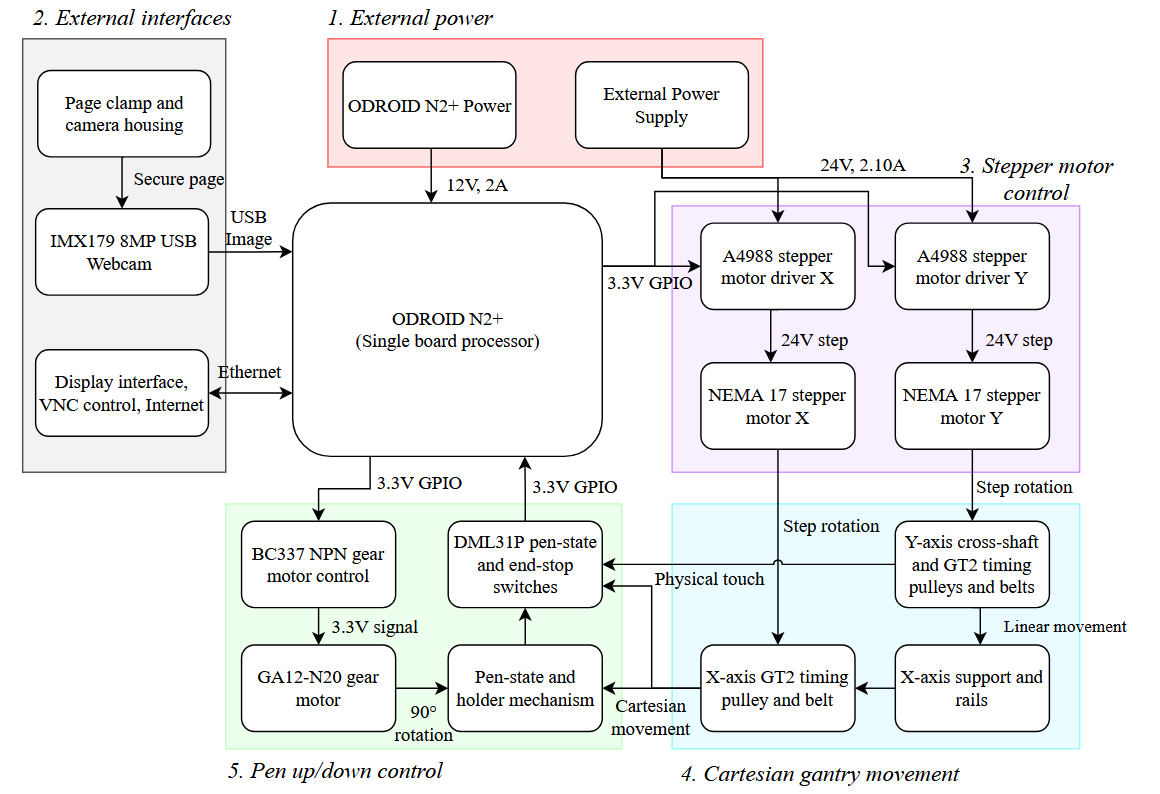
\includegraphics[width=0.96\linewidth]{Evidence/user_hardware_diagram_input.png}
\caption{Hardware system block diagram supplied by the author. The detailed controller pins, signal levels and power connections are listed in Table~\ref{tab:des-pin-map}.}
\label{fig:des-hardware-system}
\end{figure}
\FloatBarrier

\noindent\textbf{1. External power.} Separate supplies power the ODROID and the 24~V motor rail. The ODROID's dedicated 3.3~V supply pin powers the driver logic and pen motor; its GPIO pins provide control signals.

\noindent\textbf{2. External interfaces.} The page clamp holds the handwriting beneath the IMX179 USB camera, which sends images to the ODROID. The network provides interface access and remote control.

\noindent\textbf{3. Stepper motor control.} The ODROID sends STEP and DIR signals to the two A4988 drivers. Each driver regulates winding current from the 24~V rail to rotate its NEMA~17 axis motor.

\noindent\textbf{4. Cartesian gantry movement.} GT2 pulleys and belts convert motor rotation into linear X--Y motion along the rails. The Y-axis cross-shaft mechanically couples the two side belts to move the supported X-axis rail together.

\noindent\textbf{5. Pen up/down control.} A GPIO-controlled BC337 transistor switches the GA12-N20 gear motor to raise or lower the pen holder. Five switches return feedback to the ODROID: four indicate axis limits and one reports the raised pen state.

\clearpage
\begin{figure}[!ht]\centering
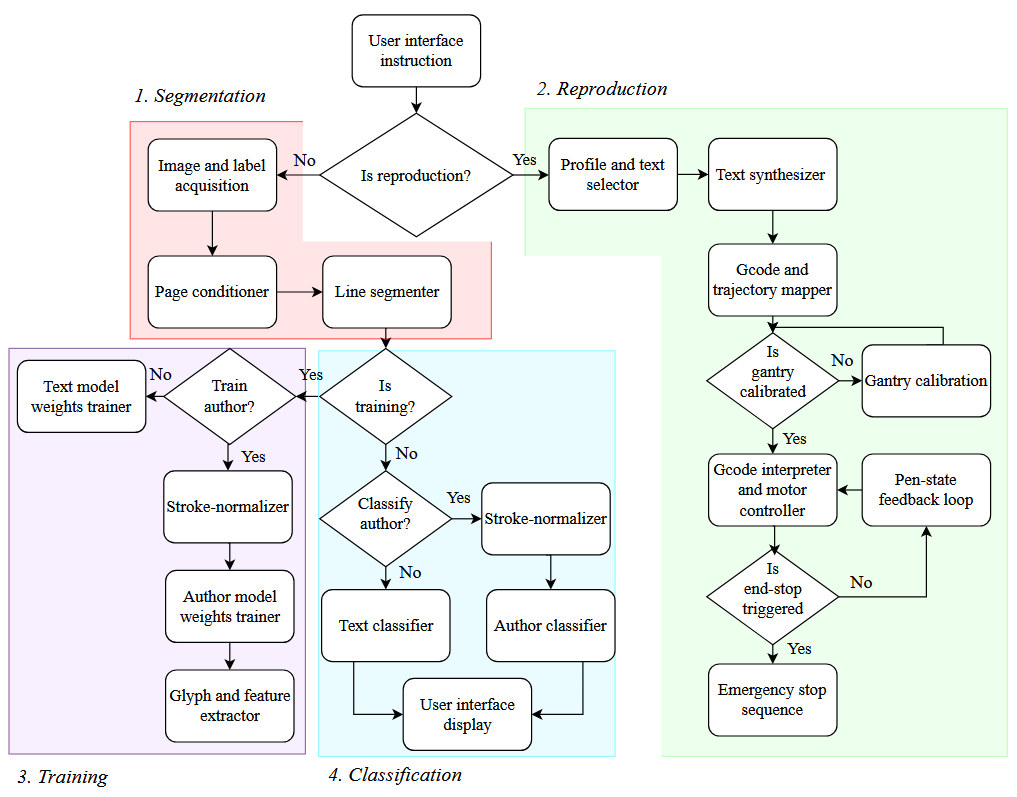
\includegraphics[width=0.98\linewidth]{Evidence/user_software_diagram_input.png}
\caption{Software system block diagram supplied by the author: (1) segmentation, (2) reproduction, (3) training and (4) classification.}
\label{fig:des-processing-system}
\end{figure}
\FloatBarrier

\noindent\textbf{1. Segmentation.} For an image-processing request, the system acquires the page and any available transcript labels. The page conditioner corrects orientation and uneven illumination, and the line segmenter separates the handwriting into line crops. These crops feed either training or classification; transcript labels are needed for supervised preparation, while classification estimates unknown content.

\noindent\textbf{2. Reproduction.} A writing request selects a stored writer profile and new text. The text synthesiser arranges the profile's glyph paths and scores candidate renderings, then the trajectory mapper converts the selected layout into G-code. Once the gantry is calibrated, the interpreter converts these commands into axis and pen-control signals. Pen-state feedback coordinates lifting and lowering, while a confirmed end-stop trip invokes the stop and recovery sequence. This is a separate request from reading a page.

\noindent\textbf{3. Training.} Segmented, labelled lines prepare the text and author models. The author route first normalises stroke thickness to the selected 0.17 x-height ratio. Transcript-guided glyph and feature extraction builds the writer profiles used for reproduction. Model training and profile extraction are separate preparation tasks: their saved weights and libraries are reused during operation. Weight training takes place off-device; page processing and motion control run on the ODROID.

\noindent\textbf{4. Classification.} The text classifier reads each complete line, while the author classifier identifies its writer after stroke normalisation. The two branches represent the requested outputs; a page report can contain both recognised text and writer identity. Line-level writer evidence is pooled before the results are returned to the interface. Character boundaries for profile construction are recovered separately using known transcripts, rather than requiring isolated letters before recognition.

The numbered groups retain the proposal's functional units: acquisition implements FU~1; conditioning and line preparation implement FU~2.1--2.2; classification implements FU~2.3; weight training implements FU~2.4; and glyph extraction, storage and retrieval implement FU~2.5--2.7. G-code conversion and interpretation implement FU~2.8, linking the software to the axis drives and pen mechanism in FU~3.1--3.4.
\FloatBarrier
